\documentclass[tikz,border=10pt]{standalone}
\usetikzlibrary{positioning}
\usepackage{kotex} % 한국어 설정

\begin{document}
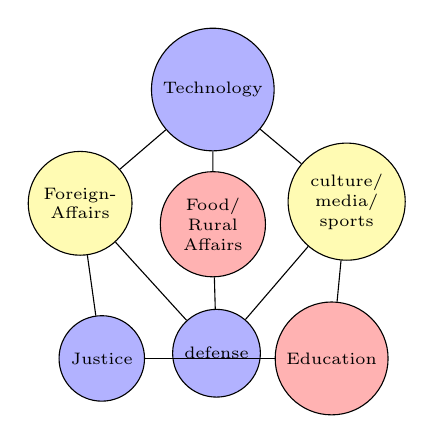
\begin{tikzpicture}[node distance=2cm]
  \tikzset{vertex/.style = {shape=circle,draw,minimum size=2.5em, align=center}} % 노드 스타일 설정

  % 노드들
  \node[vertex, fill=blue!30, font=\fontsize{6pt}{7.2}\selectfont] (0) at (2.334,0.666) {defense};
  \node[vertex, fill=red!30, font=\fontsize{6pt}{7.2}\selectfont] (1) at (3.796,0.6) {Education};
  \node[vertex, fill=red!30, font=\fontsize{6pt}{7.2}\selectfont] (2) at (2.288,2.304) {Food/\\Rural\\Affairs};
  \node[vertex, fill=yellow!30, font=\fontsize{6pt}{7.2}\selectfont] (3) at (0.602,2.57) {Foreign-\\Affairs};
  \node[vertex, fill=blue!30, font=\fontsize{6pt}{7.2}\selectfont] (4) at (0.877,0.6) {Justice};
  \node[vertex, fill=blue!30, font=\fontsize{6pt}{7.2}\selectfont] (5) at (2.287,4.015) {Technology};
  \node[vertex, fill=yellow!30, font=\fontsize{6pt}{7.2}\selectfont] (6) at (3.987,2.591) {culture/\\media/\\sports};

  % 간선들
  \draw (6) -- (0);
  \draw (6) -- (1);
  \draw (6) -- (5);
  \draw (0) -- (3);
  \draw (0) -- (2);
  \draw (1) -- (4);
  \draw (2) -- (5);
  \draw (3) -- (4);
  \draw (5) -- (3);

\end{tikzpicture}
\end{document}

